\documentclass[]{IEEEtran}
\usepackage[utf8]{inputenc}		%UTF8 input file
\usepackage[T1]{fontenc}		
\usepackage[ngerman]{babel}
\usepackage{amsmath, amssymb}
\usepackage{eurosym}
\usepackage{hyperref}
%Für Fußzeilten
%\usepackage{stfloats}
%Bilder
\usepackage{graphicx}

%Zeilenabstände
\usepackage{setspace}


\title{Pflanzengießanlage}
%\subtitle{DIY14Pflanze}
\date{\today}
\author{ Stefan Schubäck, \and Matthias Nagl,\and Christoph Hofbauer, \and Dmitrii Cetvericov, \and Markus Fischer-Has,}

%\renewcommand{\iedlistdecl}{\settowidth{\labelwidth}{Hello}}

\begin{document}


	\maketitle
%	\tableofcontents

\begin{abstract}
Auch unter den Studenten gibt es den einen oder anderen mit einem grünen Daumen, der seine Wohnung durch ein paar Pflanzen aufgewertet hat. 
Wenn nicht das ständige Gießen wäre. 
Vor jedem längeren Urlaub stellt sich die Frage, was machen mit den ganzen Pflanzen? 
Den Nachbarn fragen und hoffen er ist da und verlässlich? 
Die Pflanzen "Absaufen" lassen und hoffen, dass die sich das Wasser einteilen? 
Beides keine zufriedenstellende Lösung. Wieso lässt man sich die Pflanze nicht selber gießen?
Aus diesen Überlegungen ist die Idee entstanden, eine Pflanze mit Sensoren auszustatten, die uns über den aktuellen Zustand informieren. 
Im Folgenden wird der Aufbau zweier Lösungen vorgestellt. 
Die erste Lösung basiert auf dem Arduino-System die einen einfachen Einstieg in Umgang mit Mikrocontroller ermöglicht. 
Der zweite Ansatz baut auf ähnliche Hardware ohne die Verwendung der Arduino Programmierumgebung. 
Dadurch wird die Verwendung von Sleep-Modi und Interrupts möglich und wird somit zu einer Low-Energy Variante des Gießsystems.  

\end{abstract}
\section{Idee}\label{refIdee}

 Die wichtigste Information in dieser Hinsicht ist die Bodenfeuchtigkeit im Topf der Pflanze. 
 Neben dieser können noch weitere Informationsquellen herangezogen werden, die über das Wohlbefinden der Pflanze Aufschluss geben. 
 Hierunter fallen unter anderer der Nährstoffgehalt der Erde, die Temperatur an der Wurzel und die Luftqualität im Umfeld der Pflanze.

%Gießsystem WG


\section{Eingrenzung}
Es lassen sich viele Faktoren finden, die einen Einfluss auf das Wohlbefinden eine Pflanze haben. 
Hierunter fallen die Bodenfeuchtigkeit im Topf der Pflanze, die durchschnittliche Sonneneinstrahlung, der Luftqualität sowie der Nährstoffgehalt des Bodens. 
Diese nicht abschließende Aufzählung zeigt, dass eine Eingrenzung der zu untersuchenden Faktoren notwendig ist um das Projekt in der gegeben Zeit fertigzustellen.
Auch in Hinblick des Einsatzgebietes gibt eine Vielfalt von unterschiedlichen Möglichkeiten wie z.B. Einpflanzenbetrieb oder Mehrpflanzenbetrieb sowie Indoor oder Outdoor. 
Im Rahmen des Projekts werden demnach folgende Eingrenzung vorgenommen.

\begin{itemize}
	\item Die Bodenfeuchtigkeit wird abgeleitet aus der Widerstandsänderung einer Messgabel die sich im Erdreich der Pflanze befindet. Die Widerstandsänderung ergibt sich aus der Änderung des Wassergehalts der Erde.
	\item Das System soll für eine alleinstehende Pflanze aufgebaut werden. 
	\item Das Einsatzgebiet wird im Innenbereich sein. Dadurch fallen Einschränkungen bzgl. Witterungs"-beständigkeit sowie für die Energieversorgung weg.
	\item Das System wird so ausgelegt, dass es über ein Netzteil ständig mit Strom versorgt wird.
	\item Das System soll über eine Drahtlose Verbindung eingestellt werden können. Diese Einschränkung gilt nur für die Arduino Variante, da in der Sparversion auf die Kommunikation verzichtet wird. Hier wird die Einstellung direkt im Code vorgenommen.

\end{itemize}

Weitere Ideen wie z.B. eine Autarke Lösung mit Batteriebetrieb, ein \emph{Mehr-Pflanzenbetrieb} oder ein System für den Garten wurden zwar diskutiert aber wegen dem erhörten Zeitaufwand und begrenzten Budgets nicht weiter verfolgt. 
Im folgenden wird Arduino Version ausführlich vorgestellt. 
Die \emph{Sparversion} wird im Anschluss kurz erläutert, da viele der Funktionen grundsätzlich identisch sind wird darauf verzichtet diese erneut auszuformulieren. 

\section{Arduino Variante}
Im Folgenden beschreiben wir das Vorgehen für das Gießsystem basierend auf der Arduino Variante. 
Es wird demnach auf folgende Bereich Eingegangen.  

\begin{itemize}
	\item Zu beginn beschreiben wir verschiedenen Möglichkeiten des Wassertransports zur Pflanze.
	\item Im weiteren stellen wir das Vorgehen zur Erstellung des Gehäuses für die Elektronik dar.
	\item In Abschnitt Elektronik werden wir auf den Aufbau der Platine und die hiermit verbunden Bereiche Sensorschaltung, Stromversorgung und Kommunikation eingehen.
	\item Anschließend gehen wir auf das Programm ein, mit dem entschieden wird wann der Zeitpunkt erreicht ist um die Pflanze zu gießen sowie.
	\item Abschließend werden die verwendetet Materialien aufgelistet und
	\item eine kurzer Kostenplan vorgestellt. 
	
\end{itemize}

\subsection{Wassertransport}
Um den Einsatzbereich so flexibel wie möglich zu halten haben wir uns für ein Pumpensystem entschieden. 
Dadurch ist die Anordnung der Pflanze relativ zum Wassertank nicht relevant. 
Der hiermit einhergehen erhöhte Strombedarf ist zu verkraften, da unser System nicht auf Batterien angewiesen ist.

Für den Wassertransport haben wir uns für eine Zahnradpumpe entschieden.
Diese setzte sich gegenüber anderen Lösungen vor allem wegen ihrer selbstsaugenden Eigenschaft durch.
Selbstsaugend bedeutet, dass eine mit Luft gefüllten Wasserleitung und Pumpe Wasser ansaugen und fördern kann. 
Als Alternativen wurden Ventile und Kreiselpumpen angedacht.
Die Kreiselpumpe konnte trotz dem geringeren Stromverbrauch und geringerem Geräuschpegel nicht durchsetzen. 
Noch weniger Strom und Lärm verursachen Ventile, die aber auf gespeicherte Energie angewiesen sind.  
Entweder durch Druck im Wassertank oder durch Erhöhung des Tankes über den Ausfluss. 
Auf Grund der Wahl der Zahnradpumpe kann ein 4 mm Schlauch zur Förderung des Wassers genutzt werden. 
Das Gefäß ist frei wählbar deswegen wurde hier ein fünf-Liter-Weinballon gewählt. 
In den der Schlauch gesteckt wird. 
Auf der anderen Seite wird das Schlauchende mit einem durchbohrten Kantholz in der Pflanzenerde befestigt.
	
Die Nachteile der Zahnradpumpe (Stromverbrauch und Lärm) haben wir dadurch minimiert, dass das Gießsystem über ein Netzgerät mit Strom versorgt wird ist der erhöhte Stromverbrauch zwar unschön aber vertretbar. 
Um den Geräuschpegel zu minimieren wird über einen Helligkeitssensor verhindert, dass in der Nacht gegossen wird. 
Dies wird im Abschnitt~\ref{sensorik} näher erläutert.
	
\begin{table}
	\centering

		\onehalfspacing
	\footnotesize
	\caption{Vergleich Wasserpumpen und Ventil}
	\label{Vergleich zwischen Wasserpumpen und Ventil}
		\begin{tabular}{|l|lll|}
		\hline
		\textit{Eigenschaft} & \textit{Zahnradpumpe} & \textit{Kreiselpumpe} & \textit{Ventil} \\
		\hline
		Selbstsaugend	&ja	&nein &nein\\		
		Lautstärke		&sehr laut	&mittel laut	&leises Klacken\\
		Stromverbauch	&@12V 2,8A	&@12V 0,6A	&@12V 80mA\\
		Förderleistung	&gering		&groß		&keine eigene\\
		Preis			&2,95 \euro	& 2,95 \euro	&	4,95 \euro\\
		\hline		
		\end{tabular}
		
\end{table}	
	
	
	
\subsection{Gehäuse}
	Das Gehäuse wurde so konzipiert, dass es möglichst klein ist aber genügend Platz für die Elektronik bietet.
	Im Gehäuse verbaut sind:
\begin{itemize}
	\item das LCD-Display
	\item zwei Taster zur Steuerung der Displayanzeige und zum manuellen Gießen
	\item der Photowiderstand zur Messung der Helligkeit (platziert zwischen den Tastern)
	\item Stromschluss auf der linken Seite
	\item Ausgänge für die Pumpe und den Feuchtigkeitssensor auf der rechten Seite

\end{itemize}	

	\begin{figure}[!h]
	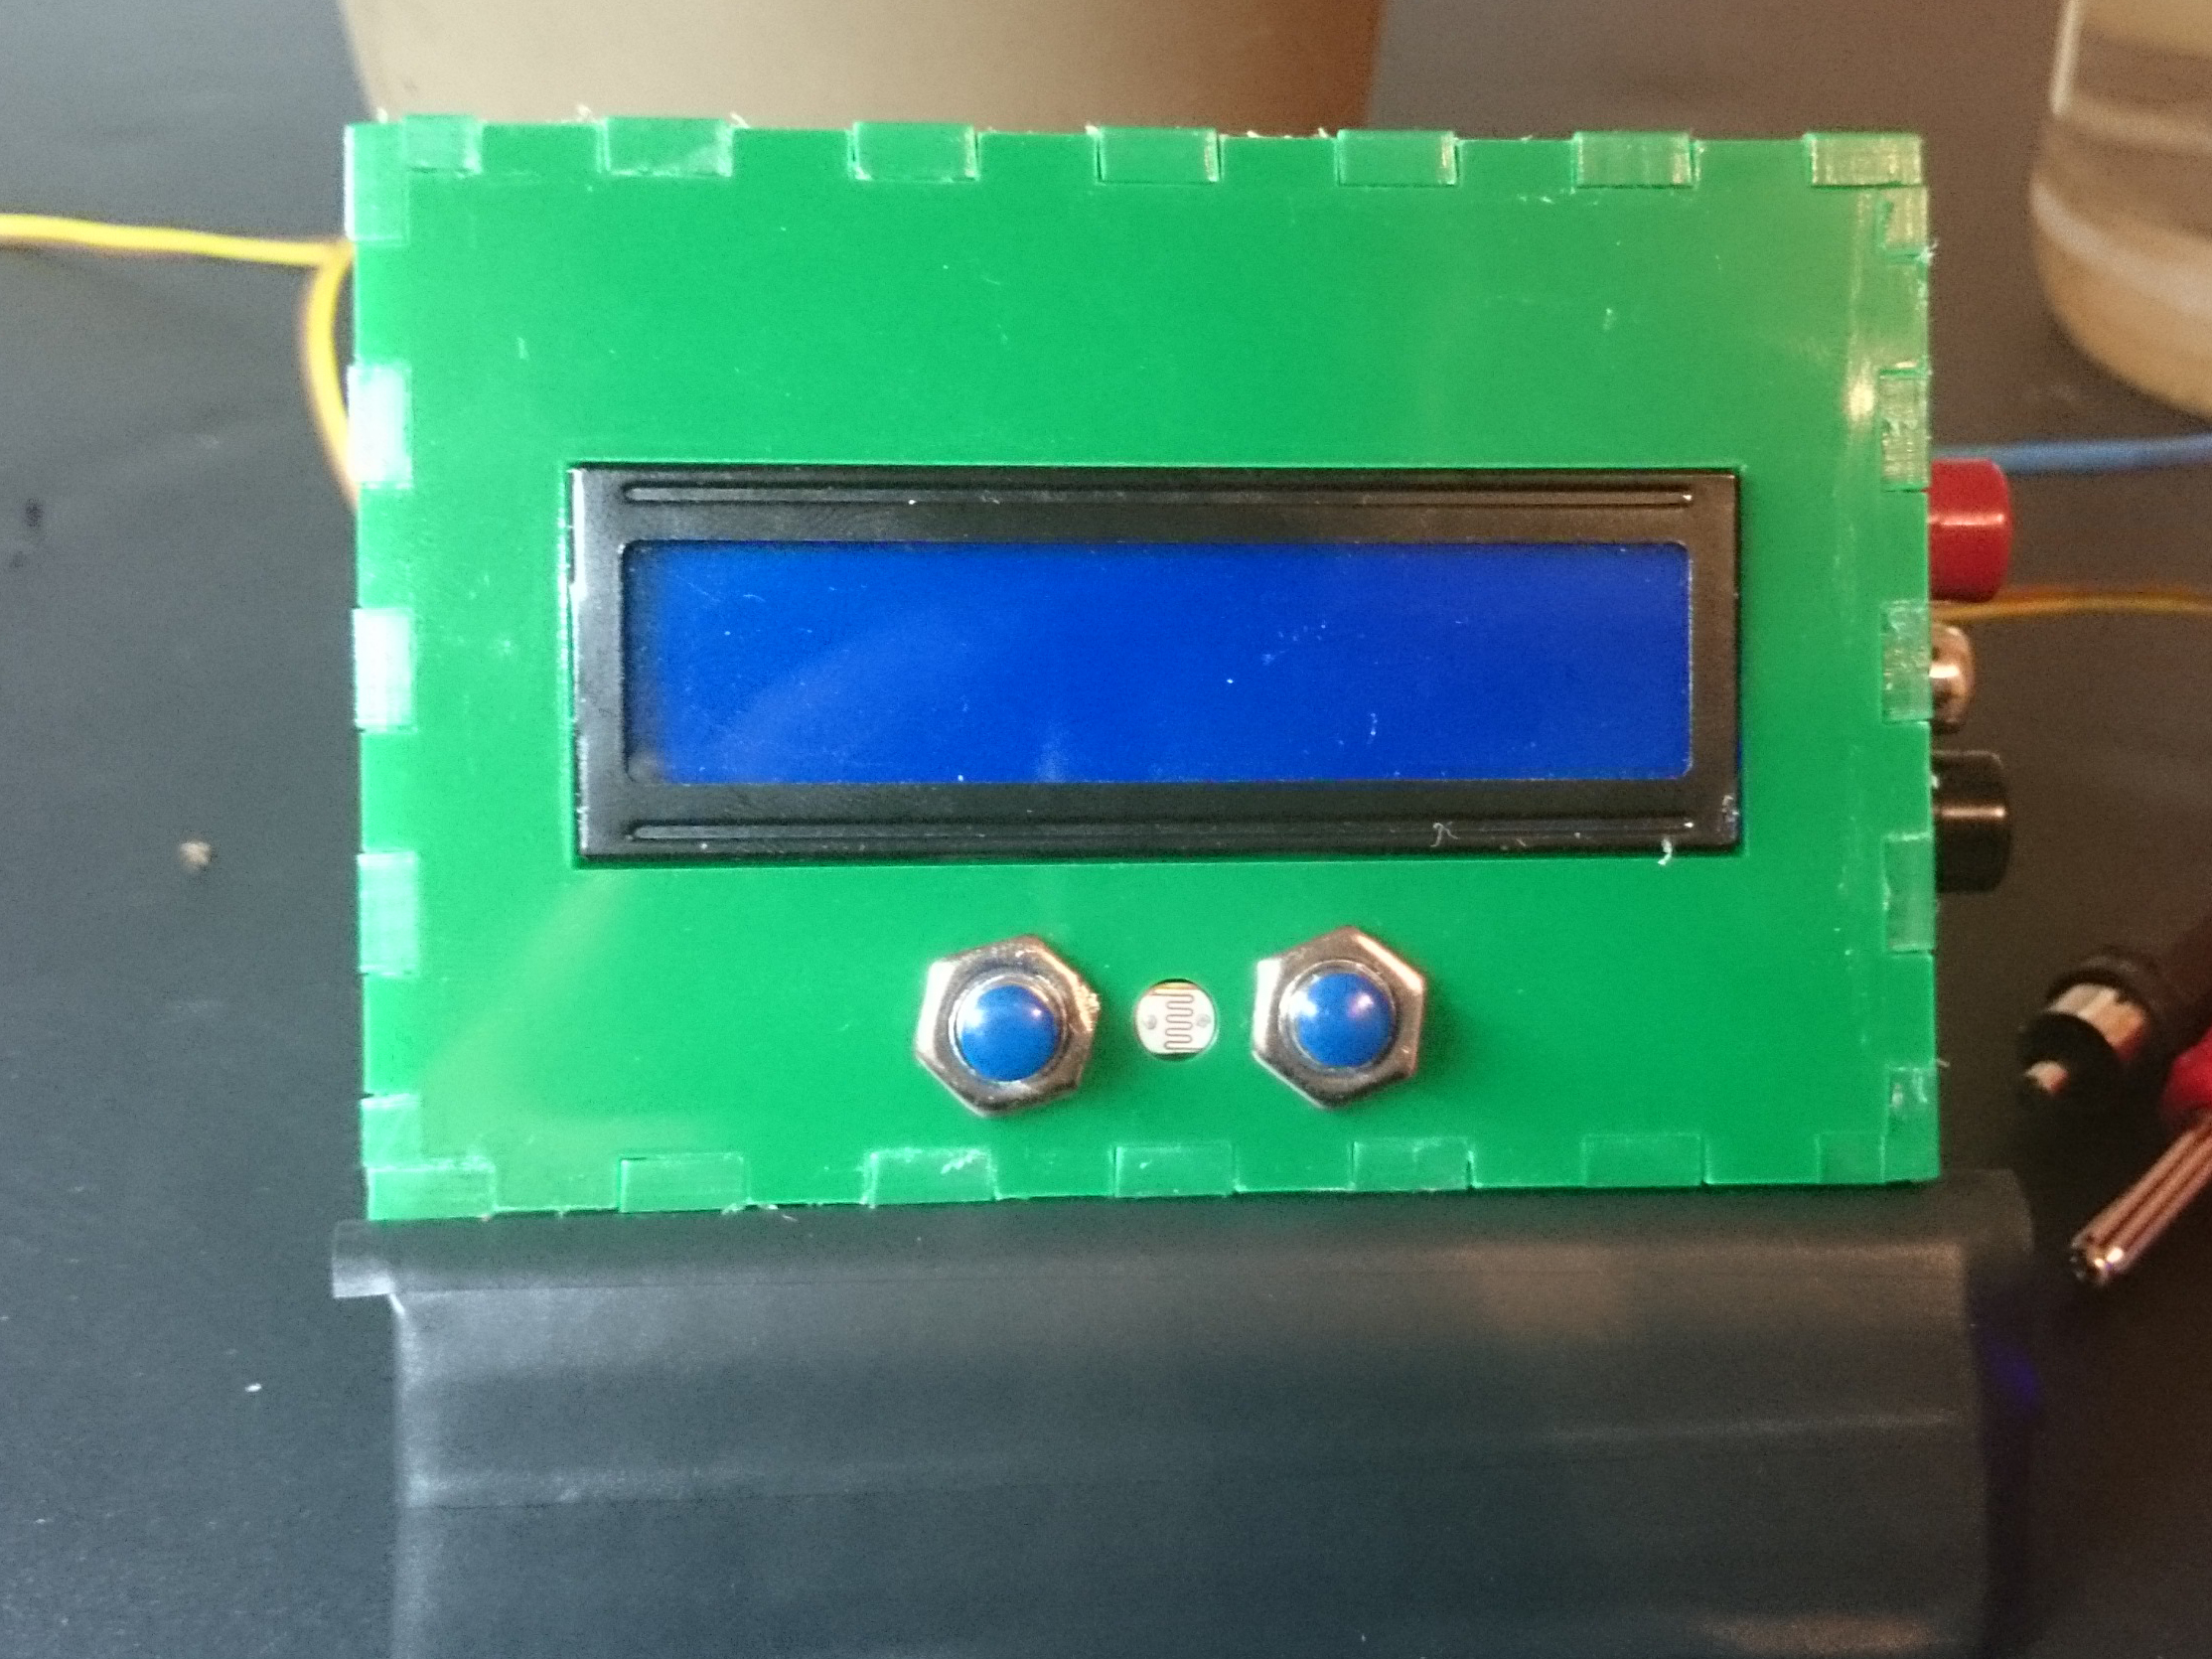
\includegraphics[width=0.8\linewidth]{bilder/_boxFron1.jpg}	
	\caption{Gehäuse Frontansicht}
	\label{fig-Gehäuse}
	\end{figure}
	
Das Gehäuse wurde in FabLab Erlangen mit einem Lasercutter gefertigt. 
Für das Design des Gehäuses wurde der BoxMaker\footnote{ \href{http://boxmaker.connectionlab.org/}{http://boxmaker.connectionlab.org/}} verwendet. 
Das Gehäuse besteht aus grünen 3mm dicken Acrylglas.
	
\subsection{Elektronik}
	Im folgenden wird der Aufbau der Version~1.0 der Arduino Variante vorgestellt. 
	Während des Aufbaus, vor allem aber während der Testphase sind ein paar Probleme aufgetreten die dazu geführt habe, dass eine neue Version~1.1 erstellt werden musste. 
	Diese neue Version ist jedoch aus zeitlichen Gründen noch nicht komplett aufgebaut. 
	Ein neues Layout wurden bereits erstellt und die Software ist so angepasst worden, dass diese ohne größere Änderungen übernommen werden kann. 
	Daher wird wird die Funktionsweise auf Basis der Version~1.0 erläutert, an gegebener Stelle wird auf die Anpassungen eingegangen die bereits umgesetzt wurden bzw. noch in Planung sind. 

			
\subsubsection{Sensorik} \label{sensorik}
Für den Helligkeitssensor wird ein einfacher Photowiderstand verwendet, der über einen Spannungsteiler an einem der Analogen Pins des Arduino Bords angeschlossen ist. Der Pin verfügt über einen 10\,Bit AD Konverter und gibt demnach einen Integerwert von 
0\,-\,1023 zurück.
Der Bodenfeuchtigkeitssensor bestimmt den Wassergehalt des Bodens über eine Widerstandsmessung zwischen den zwei Zinken einer Messgabel. 
Je mehr Wasser im Erdreich vorhanden ist, desto kleiner ist der gemessene Widerstand im Boden.

\begin{figure}[!h]
	\centering
	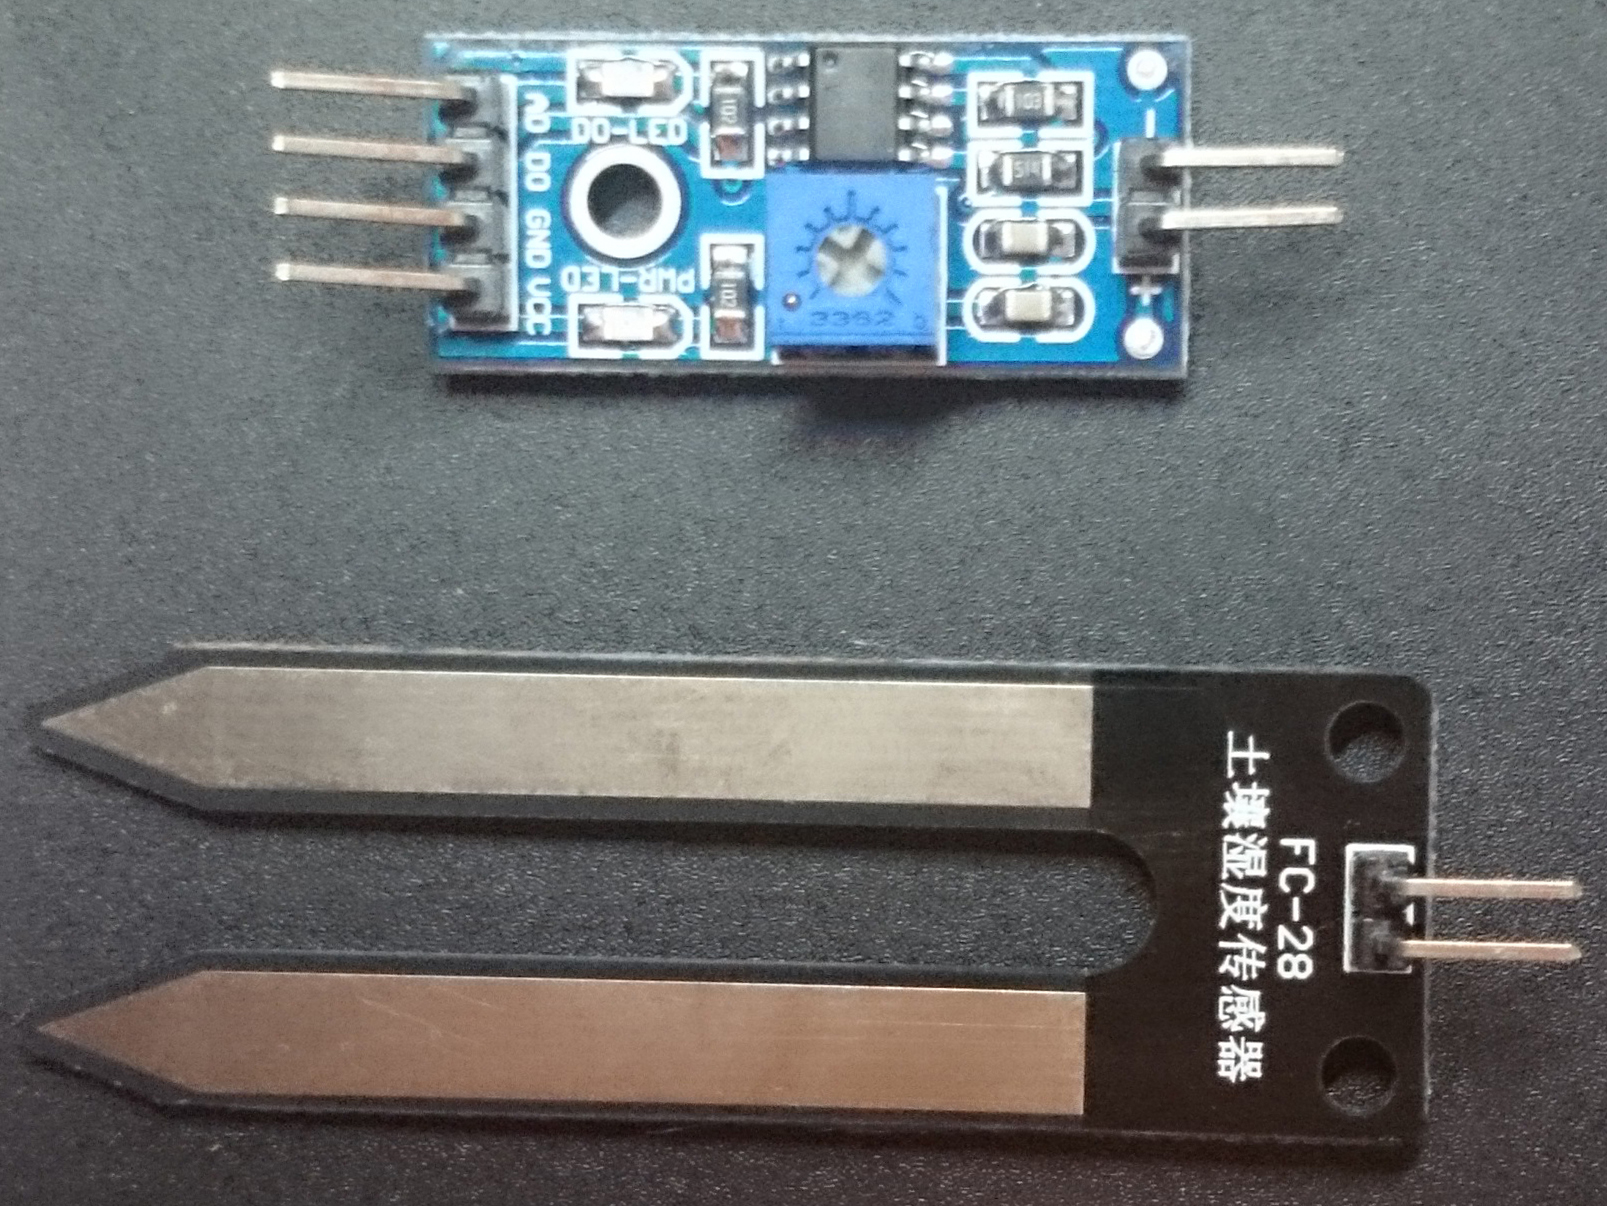
\includegraphics[width=0.8\linewidth]{bilder/_feuchteSensor1.jpg}
	\caption{Feuchtigkeitssensor mit Vorschaltung}
	\label{fig-SensorVorschaltung}
\end{figure}
Der Feuchtigkeitssensor benötigt keine weiteren Schaltelemente, da er über eine eine Vorschaltung verfügt, in der ein Spannungsteiler bereits verbaut ist. 
Abbildung \ref{fig-SensorVorschaltung} zeigt den verwendeten Sensor und die Vorschaltung. 
Es ist möglich sowohl den Analogen Wert, oder ein Digitales Signal auszuwerten. 
Das Digitale Signal liefert einen Null"-wert solange ein Grenzwiderstand nicht überschritten wird. 
Über ein  Potentiometer(1) lässt sich diese Grenze Einstellen. 
Wegen des schlechten Zugangs zum Potentiometer im eingebautem Zustand wird der Digitale Output nicht verwendet, sondern der Analoge Messwert selbst ausgewertet und mit einer Variablen im Mikrocontroller abgeglichen.
		
\emph{Anpassung zu Version~1.1:}
Leider zeigte sich, dass nach nur 48 Stunden Dauermessung die Gabel erhebliche Korrosion erlitten hat, Abbildung \ref{fig-SensorVergleich} zeigt dies deutlich.
Die Vorschaltung sieht keine Abschaltung des Messprozesses vor noch eine Umpolung der Gabel. 
Deswegen muss die gesamte Vorschaltung stromlos geschaltet werden, um das Auflösen des Sensors zu verlangsamen. 
Hierfür haben, wir für die Version~1.1, eine Transistorschaltung für den Sensor eingefügt. 
Über diese Schaltung wird die Vorschaltung des Feuchtigkeitssensor stromlos geschaltet und der Sensor ist nur für eine Messung unter Strom. 
Eine Umpollung der Messgabel ist damit leider nicht möglich. 
Dies kann jedoch relativ einfach gelöst werden, indem der Sensor alle paar Wochen \emph{manuell} umgepolt wird. 
Hierfür muss lediglich die Messgabel vom Verbindungskabel abgesteckt werden und um \begin{math}180^{\circ}\end{math} gedreht wieder verbunden werden.

\begin{figure}[!h]
	\centering
	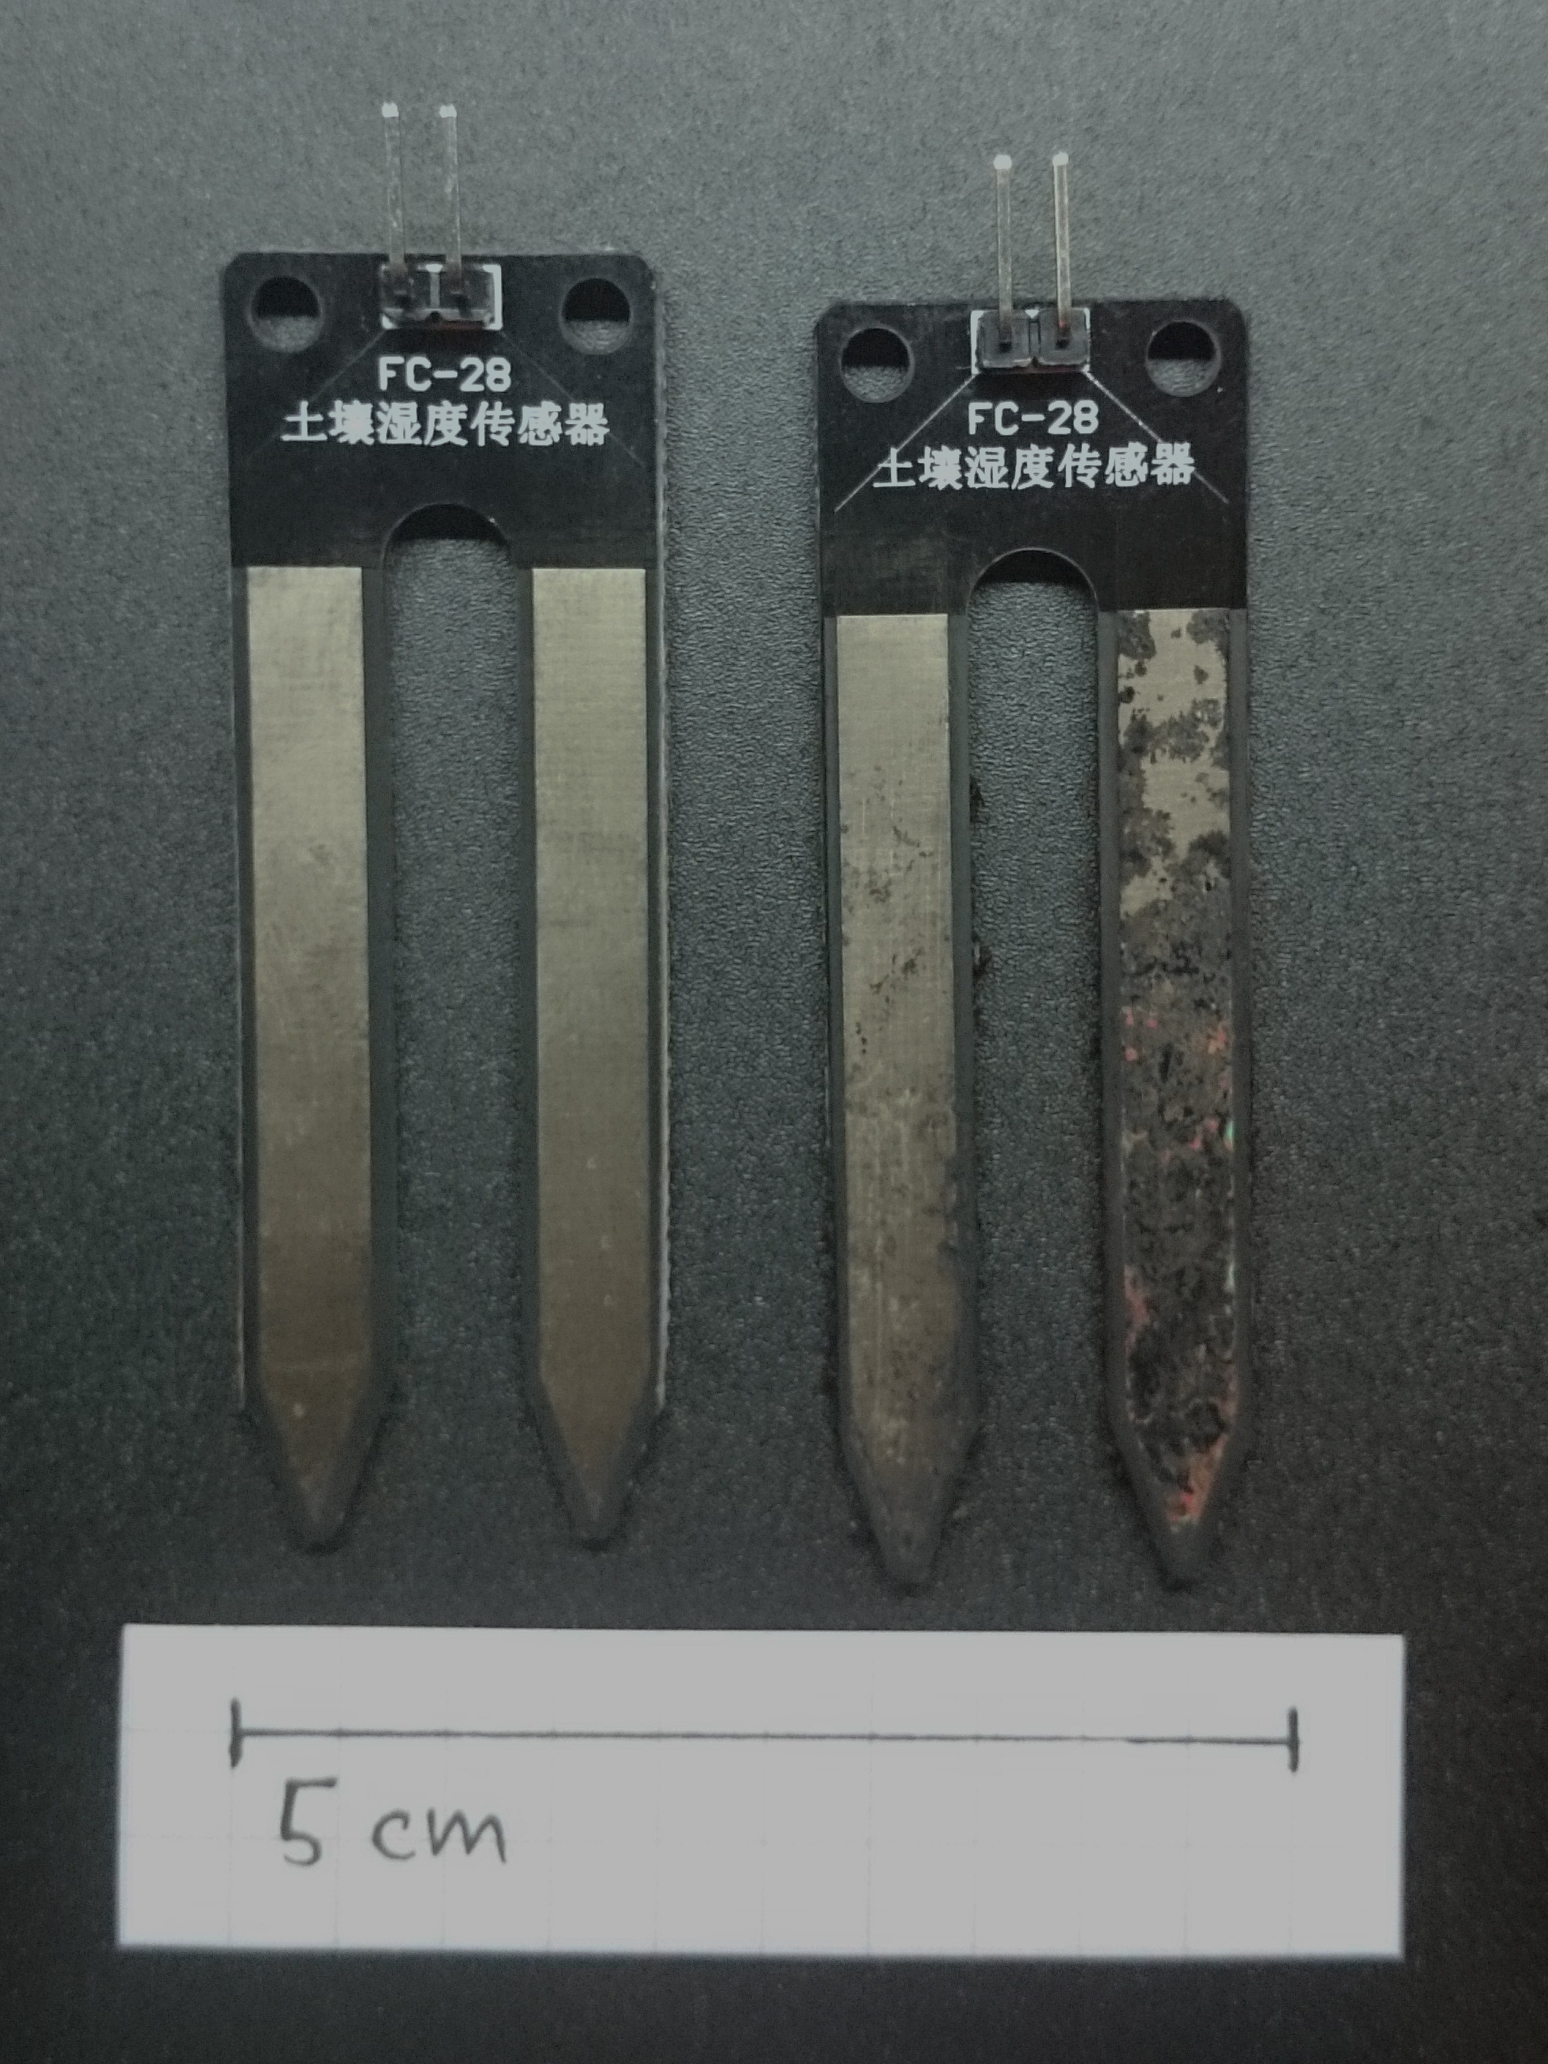
\includegraphics[width=0.8\linewidth]{bilder/_fechtesensorVergleich0.jpg}
	\caption{Vergleich neuer Sensor und Sernsor mit 48h Dauerbetrieb}
	\label{fig-SensorVergleich}
\end{figure}

\subsubsection{Kommunikation}
Ziel der Kommunikation ist es, eine Möglichkeit zu haben das Gießsystem im laufenden Betrieb einzustellen. 
Jede Pflanze braucht unterschiedlich viel Wasser. 
Genauso hat die Zusammensetzung der Erde einen Einfluss auf den gemessenen Widerstand des Feuchtigkeitssensors. 
Diese Werte müssen daher für jede Pflanze extra einstellbar sein. 
Wir haben uns für eine Drahtlose Kommunikation entschieden und haben uns auf den XBee Standard geeinigt. 
Das XBee Modul wurde direkt, d.h. ohne Verwendung eines \emph{Arduino XBEE-Shields}, mit dem Arduino verbunden. 
Hierfür ist es notwendig einen Pegelwandlung von 5\,V auf 3,3\,V vorzunehmen, da die Logik-Pins des XBee Moduls nicht mit 5\,V betrieben werden können. 
Bei dieser Pegelschaltung ist uns in Version~1.0 ein Fehler unterlaufen, weswegen wir keine Verbindung mit ein Computer aufbauen konnten. 
Der Fehler war, dass für die Pegelwandlung für den Anschuss TX, der Transistor falsch beschaltet wurde. 
Auf dem \emph{Gate} des Transistors wurde das falsche Spannungspotential geschalteten. 
Dieser Fehler wird für die Version~1.1 behoben und noch getestet.

\begin{figure}
	\centering
	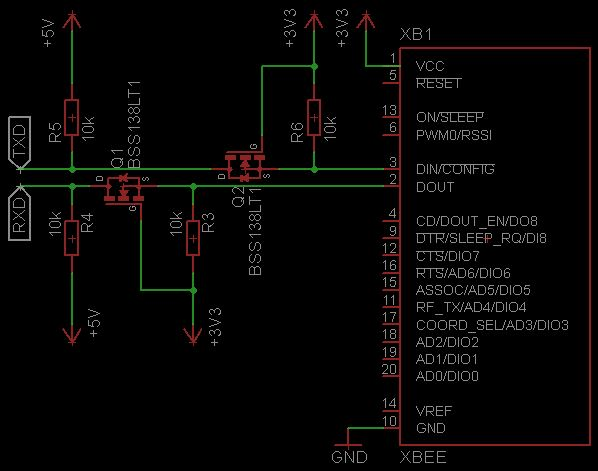
\includegraphics[width=0.8\linewidth]{bilder/v1SchaltplanXbee.jpg}
	\caption{Pegelwandler mit Small-Signal-Transistor BSS138W }
	\label{fig-Pegel}
\end{figure}
		
Die zweite Schnittstelle mit dem Menschen wird über ein Display ermöglicht. 
Hier lässt sich über einen Taster die einzelnen Variablen mit ihren aktuellen Werten Überprüfen. 
Bei dem Display Handelt es sich um ein 2 Zeiliges LCD-Display mit jeweils 16 Zeichen. 
Die Kommunikation zwischen Display und Mikrocontroller wird über eine I2C-Schnittstelle bewerkstelligt. 
Hierfür haben wir die frei verfügbare LiquidCrystal\_I2C Libary von fderbrabander verwendet.\footnote{\href{https://github.com/fdebrabander/Arduino-LiquidCrystal-I2C-library}{https://github.com/fdebrabander/Arduino-LiquidCrystal-I2C-library}}
	
	
\subsubsection{Stromversorgung}

Eine Stromversorgung über USB ist nicht möglich, da die Pumpe in Voll"-last 12\,V und außerdem 2,8\,A benötigt. 
Deswegen muss auf eine leistungsfähigere Energiequelle gesetzt werden.
Wir entschieden uns für Netzteile mit 12\,V Ausgangs"-spannung um die Pumpe direkt anschließen zu können. 
Um den Strom der Pumpe zu begrenzen haben wir einen \begin{math}5~\Omega\end{math} Lastwiderstand in Reihe geschaltet.
Dies führt zu geringerer Leistungsaufnahme und deutlichen Geräusch"-minderung.
Die Ansteuerung der Pumpe über dem Mikrocontroller wurde über eine Transistorschaltung gelöst (Ziffer 1 in Abbildung \ref{fig-Schaltplanv1.0}).
Es ist zu überlegen, den Transistor und den Mikrocontroller über eine Schutzdiode über die Anschlüsse \emph{VENTIL-1} und \emph{VENTIL-2} vor Überspannung zu schützen, die beim Abschalten der Pumpe auftreten können. 
 

\begin{figure*}
	\centering
	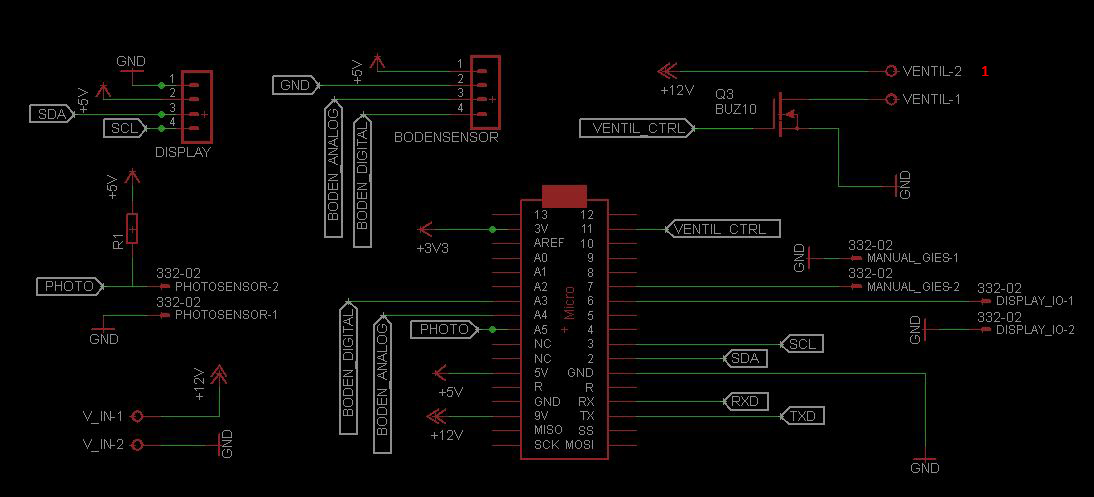
\includegraphics[width=0.9\linewidth]{bilder/v1SchaltplanMicro0.JPG}
	\caption{Schaltpaln V1.0 mit Arduino Micro}
	\label{fig-Schaltplanv1.0}
\end{figure*}

\subsection{Programm}
	

	Die Aufgaben des Mikrocontrollers sind die folgenden:
		\begin{itemize}
			\item Messung der Feuchtigkeit
			\item Messung der Helligkeitssensor
			\item Vergleich der Messwerte mit den festgelegten Grenzen
			\item Ansteuerung der Pumpensystem
			\item Ausgabe der wichtigen Variablen auf dem Display über Taster
			\item Manuelles Gießen über Taster
			\item Display Hintergrundbeleuchtung abschalten nach 60  Sekunden
			\item Übertragen/Empfangen von Einstellungen über xBee Verbindung
		\end{itemize}
		
	In der ersten Version wurden die Messungen andauernd durchgeführt. 
	Wie aber bereits oben erläutert hat dies zu einer starken Korrosion am Feuchtigkeitssensor geführt. 
	Aus diesem Grund wurde für die Version~1.1 einige Änderungen eingeführt. 
	Anstelle bei jedem Aufruf der Loop() Methode eine Messung durchzuführen wird nur noch alle 4 Stunden eine Messung vorgenommen. 
	Ist das Intervall abgelaufen wird der Feuchtigkeitssensor über eine Transistorschaltung angeschaltet und anschließend ausgelesen. 
	Dadurch ist der Sensoren nur noch für einen kurzen Zeitraum unter Strom, was die Lebensdauer des Feuchtigkeitssensor verlängert.
		
	
	%\subsection{Setuptool}
	Da die Erde in jeder Pflanze eine andere Zusammensetzung hat und jede Pflanze unterschiedlich viel Wasser benötigt ist es notwendig die Grenzwerte für die Feuchtigkeit und die Wassermenge einzustellen. 
	Hierfür gibt es ein Cmd-Tool welches über die 
	

	
\subsection{BOM - Bill of Matirial}
	
\subsection{Kostenplan}
 Durch die geringen Kosten pro Entwicklungsstufe hatten wir genügend Geld um mehrere Iterationsstufen  zu durchlaufen.
 Deswegen benötigten wir für die gesamte Entwicklung etwas über hundert Euro.
 Ein einzelnes Modul kann für etwa 45\,\euro\ nachgebaut werden. 
 Die Kosten setzen sich nach Tabelle\,\ref{Kosten für eine Giessanlage} zusammen.
 
 Nicht berücksichtigt sind das Wassergefäß, die zwei \begin{math}4mm\end{math}\,-Schlauch"-stücke und Befestigung in der Pflanze.
 Bei diesen handelt es sich um Reste oder Lagerfunde die von Wert von unter 1\,\euro\ sind. 
 
\begin{table}[h]
	\centering
	\onehalfspacing
	\footnotesize
	\caption{Kosten für eine Gießanlage}
	\label{Kosten für eine Giessanlage}
		\begin{tabular}{|l|ll|}
			\hline
\textit{Bauteil} & \textit{Kosten} & \textit{Bezugsquelle} \\
\hline
Arduino Nachbau & ca. 3 \euro & ebay \\
LCD-Display & ca. 5 \euro & ebay\\
Bodensensoren & ca. 2 \euro & ebay \\
Zahnradpumpe & 2,95 \euro & Pollin \\
XBee &  23,55 \euro & Reichelt \\
Hauptplatine & ca. 6 \euro & FabLAB \\
Gehäuse	& ca. 4 \euro & FabLAB \\

\hline
Gesamt: & ca 45 \euro & \\
\hline
\end{tabular}
\end{table}

	
	
\section{Sparversion}
	Um Strom zu sparen, die Größe zu schrumpfen und Kosten günstiger zu werden, haben wir die \glqq Sparversion\grqq entwickelt.
	In dieser Variante der Gießanlage wurde die Anlage auf das wesentlichste beschränkt,das Gießen.
	Sie wurde so konzipiert, dass sie genau auf eine Pflanze zugeschnitten ist.
	Sie kann nur durch erneutes Programmieren auf andere Pflanzen und Böden angelernt werden. 	
		
	\subsection{Aufbau}
	In dieser Version wird auf das Display und die Kommunikation verzichtet.
	Dadurch wird viel der Verkabelung gespart, außerdem lässt sich die Hauptplatine deutlich kleiner gestalten.
	Der Wegfall zu weniger Platz"-bedarf des Systems führt und damit in ein kleineres Gehäuse passt.
		
	\subsection{Elektronik}
	Durch das wegfallen der XBee Platine und deren Beschaltung wird das 3,3\,V Netz nicht mehr benötigt.
	Dadurch reduziert sich die Größe der Hauptplatine auf \begin{math} 55 mm \times 32 mm \end{math}.
	Dies entspricht nicht nicht mal der Hälfte der Fläche der Version 1.1 mit \begin{math} 56 mm \times 65 mm \end{math}.
	
		
	\subsection{Logik}
	Um weiter Stromsparen zu können wurde diese Version nicht mit Arduino, sondern mit C geschriebenen Programm programmiert.
	Dies ermöglicht die Ausnutzung der Sleep Modi und die Interrupts des ATMega328. 
	Dadurch befindet sich der \glqq Arduino Nano\grqq \ hauptsächlich im Schlafmodus und verbraucht deutlich weniger Energie.
	Die Gießeinstellungen müssen auf Grund der fehlenden Kommunikation und Eingabemöglichkeiten über die Programmierung festgelegt werden.
	Durch das Wegfallen der Arduino Bootloaders, kann die Hardware nicht mehr per USB programmiert werden. 
	Mit Hilfe des AVRISP mkII \footnote{\href{http://www.atmel.com/tools/avrispmkii.aspx}{www.atmel.com/}} wird der Microcontroller direkt mit den Binärcode beschrieben.
	
	\subsection{Kostenplan}
\begin{table}[h]
	\centering
	\onehalfspacing
	\footnotesize
	\caption{Kosten für eine  Sparversion Gießanlage}
	\label{Kosten für eine Sparversion Giesanlage}
		\begin{tabular}{|l|ll|}
			\hline
\textit{Bauteil} & \textit{Kosten} & \textit{Bezugsquelle} \\
\hline
Arduino Nachbau & ca. 3 \euro & ebay \\
Bodensensoren & ca. 2 \euro & ebay \\
Zahnradpumpe & 2,95 \euro & Pollin \\
Gehäuse	& 1,50 \euro & Pollin \\
Hauptplatine & ca. 5,5 \euro & FabLAB \\
\hline
Gesamt: & ca 15 \euro & \\
\hline
\end{tabular}
\end{table}
	
	  	
	Allein auf Grund des fehlenden XBee-Moduls halbiert sich der Preis der Anlage.
	Dazu kommt das fehlende Display, das kleinere Gehäuse und günstigere Hauptplatine.
	So ist der Nachbau der Sparversion ca. 15 \euro\ teuer. 
	In Tabelle \ref{Kosten für eine Sparversion Giesanlage} sind die Kosten nochmal zusammen getragen.
	 

	
	\section{Resüme - Do's And Dont's}	


\end{document}


